\section{Large Language Models}
\begin{figure}[hbt]
    \centering
    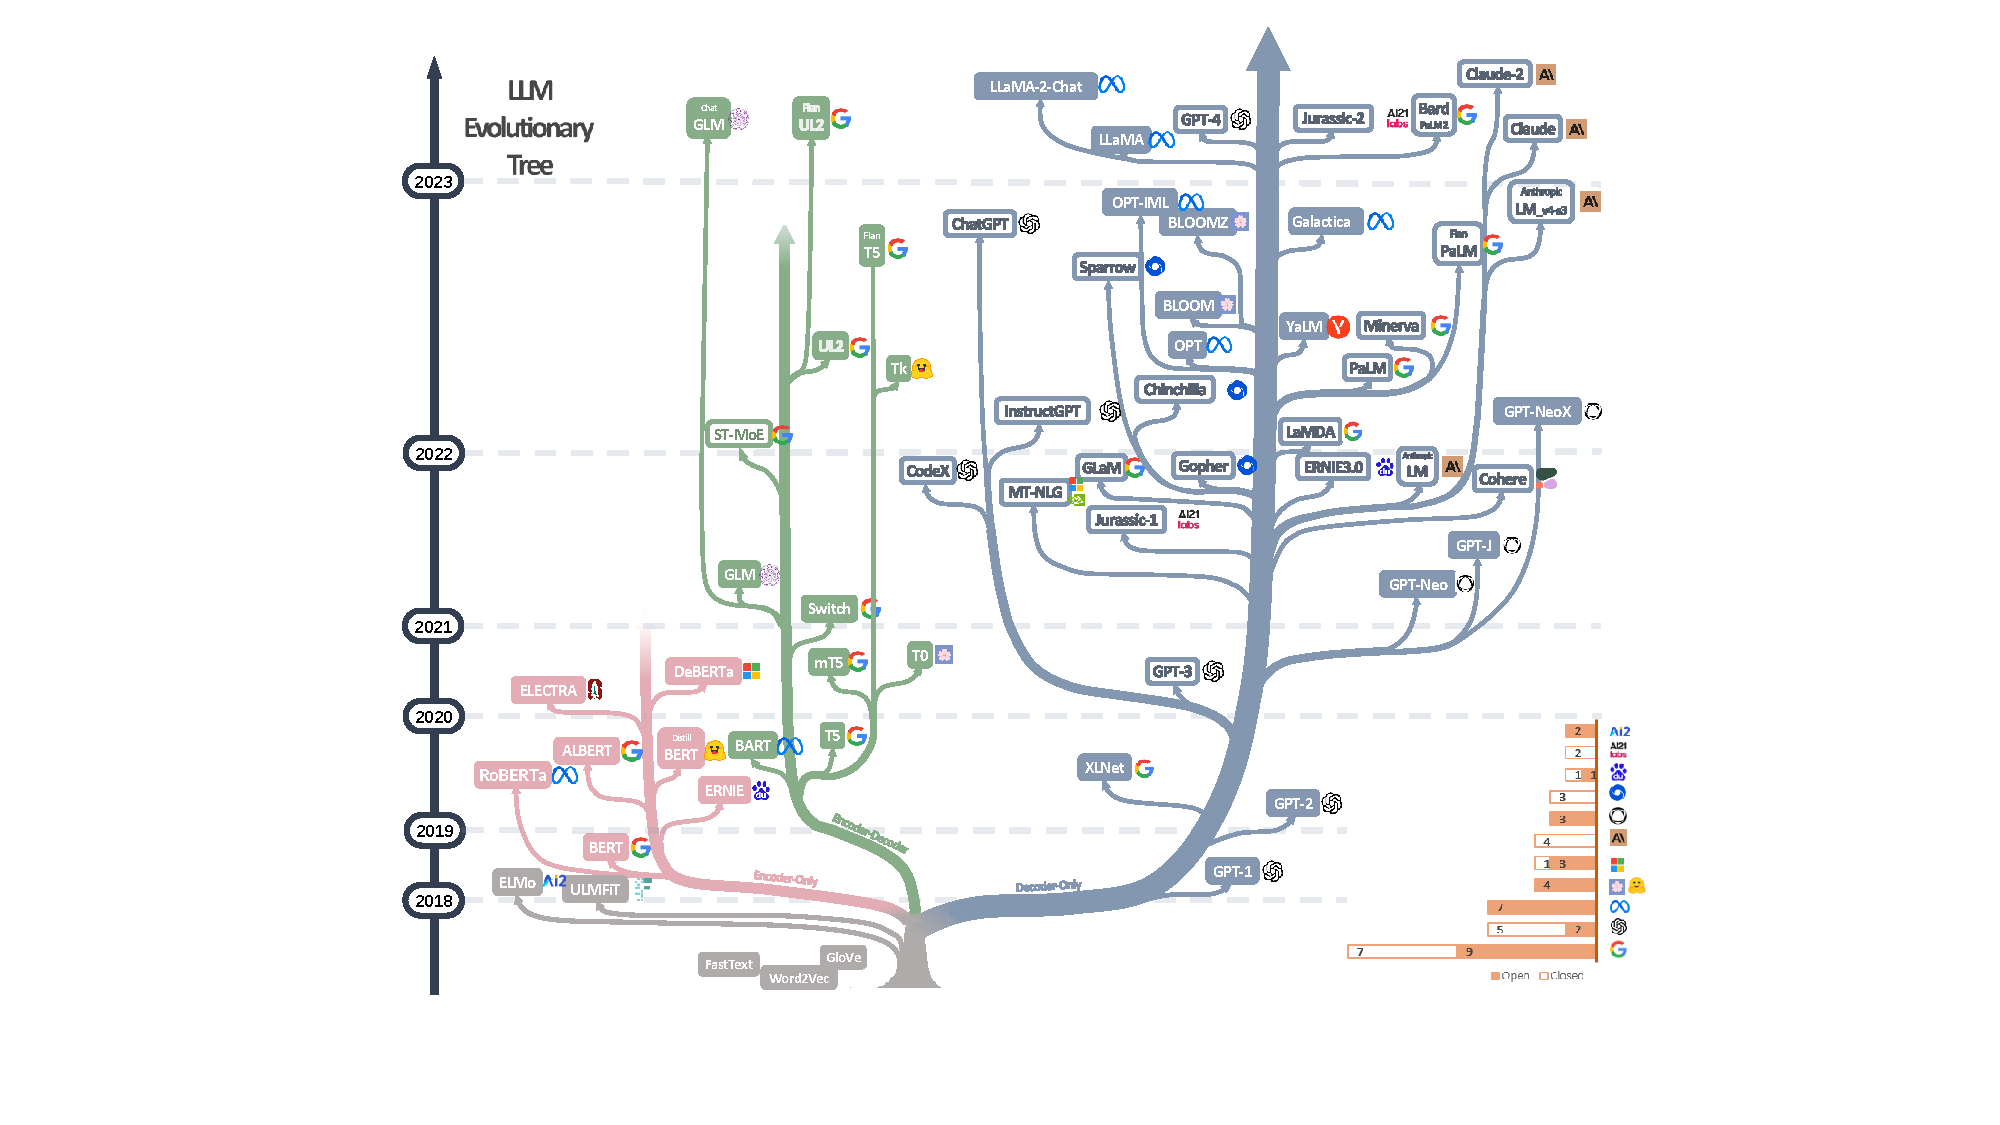
\includegraphics[width=0.95\linewidth]{theoretical-background/image/evo_tree.pdf}
    \caption{The evolutionary tree of modern LLMs traces the development of language models in recent years \cite{yang2023harnessing}}
    \label{fig:evo_tree}
\end{figure}
Large Language Models that are pre-trained on large-scale corpus have demonstrated significant potential in various natural language processing  tasks . Most LLMs are based on the Transformer design, which consists of encoder and decoder modules that are empowered by a self-attention mechanism. Based on their architecture structure, LLMs can be classified into three categories: encoder-only LLMs, encoder-decoder LLMs, and decoder-only LLMs. Figure \ref{fig:evo_tree} summarizes several representative LLMs with different model architectures, model sizes, and open-source availabilities. \\\\
\textbf{Encoder-only LLMs} are a type of Large Language Models that use only the encoder to encode the sentence and understand the relationships between words. These models are typically pre-trained by predicting the mask words in an input sentence using large-scale corpus. To resolve downstream tasks, such as text classification and named entity recognition, an extra prediction head is added to encoder-only LLMs like BERT \cite{devlin-etal-2019-bert}, RoBERTa \cite{liu2019roberta}, ALBERT \cite{lan2019albert}, and ELECTRA \cite{clark2020electra}. These models are most effective for tasks that require understanding the entire sentence.\\\\
\textbf{Encoder-decoder LLMs} adopt both the encoder and decoder module. The encoder module is responsible for encoding the input sentence into a hidden space, and the decoder is used to generate the target output text. The training strategies in encoder-decoder LLMs can be more flexible. Encoder-decoder LLMs are able to directly resolve tasks that generate sentences based on some context, such as summariaztion, translation, and question answering.\\\\
\textbf{Decoder-only LLMs} only adopt the decoder module to generate target output text. These models are trained to predict the next word in a sentence. They can perform downstream tasks with few examples or simple instructions without adding prediction heads or fine-tuning.  \cite{liu2022fewshot}. Many state-of-the-art LLMs follow the decoder-only architecture. Recently Llama-2 \cite{touvron2023llama2}, Alpaca \footnote{https://crfm.stanford.edu/2023/03/13/alpaca.html} and Vicuna \footnote{ https://lmsys.org/blog/2023-03-30-vicuna/} are released as open-source decoder-only LLMs. These models are finetuned based on LLaMA \cite{touvron2023llama} and achieve comparable performance with ChatGPT \cite{ouyang2022training} and GPT-4